\documentclass{article}

\usepackage{amsmath,amssymb}
\usepackage{tikz}
\usepackage{pgfplots}
\usepackage{xcolor}
\usepackage[left=2.1cm,right=3.1cm,bottom=3cm,footskip=0.75cm,headsep=0.5cm]{geometry}
\usepackage{enumerate}
\usepackage{enumitem}
\usepackage{marvosym}
\usepackage{tabularx}
\usepackage[amsmath,thmmarks,standard]{ntheorem}
\usepackage{mathtools}

\usepackage[utf8]{inputenc}

\renewcommand*{\arraystretch}{1.4}
\newcommand{\E}{\mathbb{E}}

\newcolumntype{L}[1]{>{\raggedright\arraybackslash}p{#1}}
\newcolumntype{R}[1]{>{\raggedleft\arraybackslash}p{#1}}
\newcolumntype{C}[1]{>{\centering\let\newline\\\arraybackslash\hspace{0pt}}m{#1}}

\DeclareMathOperator{\tr}{tr}
\DeclareMathOperator{\Var}{Var}
\DeclareMathOperator{\Cov}{Cov}
\renewcommand{\E}{\mathbb{E}}

\newtheorem{thm}{Theorem}
\newtheorem{lem}{Lemma}

\title{\textbf{Einführung in die Produktion, Hausaufgabe 8}}
\author{\textsc{Henry Haustein}}
\date{}

\begin{document}
	\maketitle
	
	\section*{Aufgabe 8}
	\begin{enumerate}[label=(\alph*)]
		\item Die einzelnen Bearbeitungsdauern sind
		\begin{center}
			\begin{tabular}{c|ccc}
				\textbf{Auftrag} & $A_1$ & $A_2$ & $A_3$ \\
				\hline
				113 & 5 & 1 & 2 \\
				114 & 7 & 2 & 10 \\
				115 & 4 & 7 & 4 \\
				116 & 6 & 9 & 4 \\
				117 & 7 & 10 & 3
			\end{tabular}
		\end{center}
		\item Die First-Come-First-Serve-Regel wurde verwendet. Die Zykluszeit beträgt 45 Zeiteinheiten und die gesamte Verspätung 9 Zeiteinheiten.
		\item Verfahren von Johnson
		\begin{center}
			\begin{tabular}{c|c|c|c||c|c||ccccc}
				& \multicolumn{3}{c||}{\textbf{Bearbeitungsmatrix}} & \multicolumn{2}{c||}{\textbf{mod. Matrix}} & \multicolumn{5}{c}{\textbf{Reihenfolge}} \\
				\textbf{Auftrag} & $A_1$ & $A_2$ & $A_3$ & $A_1^\ast$ & $A_2^\ast$ & 1 & 2 & 3 & 4 & 5 \\
				\hline
				113 & 5 & 2 & 3 & 7 & 5 & & & & & 113$^1$ \\
				114 & 4 & 8 & 5 & 12 & 13 & & 114$^4$ & & & \\
				115 & 7 & 3 & 6 & 10 & 9 & & & & 115$^3$ & \\
				116 & 8 & 8 & 4 & 16 & 12 & & & 116$^5$ & & \\
				117 & 3 & 5 & 4 & 8 & 9 & 117$^2$ & & & &
			\end{tabular}
		\end{center}
		\item Eine der folgenden beiden Bedingungen muss erfüllt sein, dann ist das 3-Maschinen-Problem auf ein 2-Maschinen-Problem reduzierbar und das Verfahren von Johnson liefert eine optimale Lösung:
		\begin{itemize}
			\item $t_{p_{2,max}} \le t_{p_{1,min}}$: $8\not\le 3$
			\item $t_{p_{2,max}} \le t_{p_{3,min}}$: $8\not\le 3$
		\end{itemize}
		Das Verfahren von Johnson liefert keine optimale Lösung.
		\item Gantt-Diagramm
		\begin{center}
			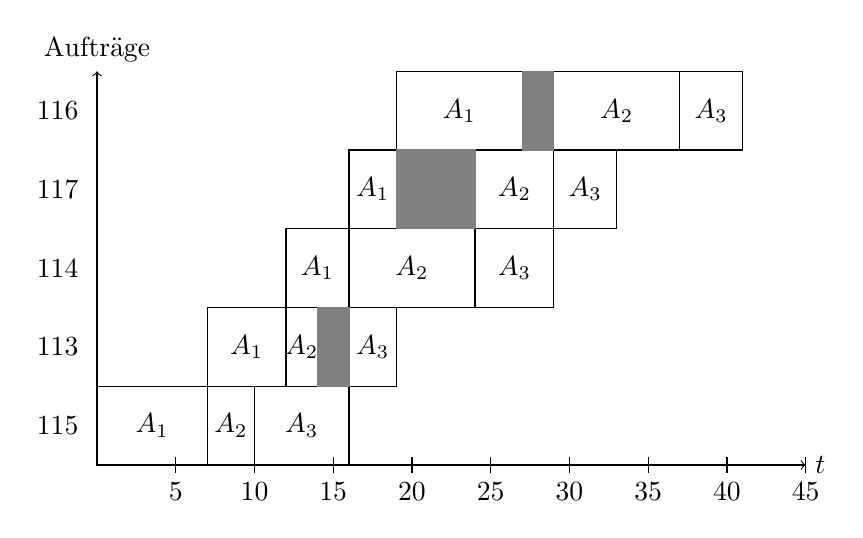
\begin{tikzpicture}
				\draw[->] (0,0) to (45/5,0) node[right] {$t$};
				\draw[->] (0,0) to (0,5) node[above] {Aufträge};
				
				\foreach \x in {5,10,15,20,25,30,35,40,45} {
					\draw (\x/5,0.1) to (\x/5,-0.1) node[below] {\x};
				}
				
				\node at (-0.5,0.5) {115};
				\node at (-0.5,1.5) {113};
				\node at (-0.5,2.5) {114};
				\node at (-0.5,3.5) {117};
				\node at (-0.5,4.5) {116};
				
				\draw (0,0) rectangle (7/5,1) node[pos=0.5] {$A_1$};
				\draw (7/5,0) rectangle (10/5,1) node[pos=0.5] {$A_2$};
				\draw (10/5,0) rectangle (16/5,1) node[pos=0.5] {$A_3$};
				
				\draw (7/5,1) rectangle (12/5,2) node[pos=0.5] {$A_1$};
				\draw (12/5,1) rectangle (14/5,2) node[pos=0.5] {$A_2$};
				\draw (16/5,1) rectangle (19/5,2) node[pos=0.5] {$A_3$};
				
				\draw (12/5,2) rectangle (16/5,3) node[pos=0.5] {$A_1$};
				\draw (16/5,2) rectangle (24/5,3) node[pos=0.5] {$A_2$};
				\draw (24/5,2) rectangle (29/5,3) node[pos=0.5] {$A_3$};
				
				\draw (16/5,3) rectangle (19/5,4) node[pos=0.5] {$A_1$};
				\draw (24/5,3) rectangle (29/5,4) node[pos=0.5] {$A_2$};
				\draw (29/5,3) rectangle (33/5,4) node[pos=0.5] {$A_3$};
				
				\draw (19/5,4) rectangle (27/5,5) node[pos=0.5] {$A_1$};
				\draw (29/5,4) rectangle (37/5,5) node[pos=0.5] {$A_2$};
				\draw (37/5,4) rectangle (41/5,5) node[pos=0.5] {$A_3$};
				
				\draw[gray,fill=gray] (14/5,1) rectangle (16/5,2);
				
				\draw[gray,fill=gray] (19/5,3) rectangle (24/5,4);
				
				\draw[gray,fill=gray] (27/5,4) rectangle (29/5,5);
			\end{tikzpicture}
		\end{center}
		Die Zykluszeit ist 41 und die Summe der Wartezeiten ist 2 + 5 + 2 = 9.
	\end{enumerate}
	
\end{document}